\section{Experimental results}
\subsection{Implementation}

{\bf Execution Summary\ } The static analysis phase computes a set of execution summaries, each representing a legal execution, which are used as the input of the dynamic analysis phase.
Each execution summary describes (i) the return value of each transaction instance and (ii) the final map state
 

In our experiments,  we have two threads running two types of transactions ($TX_1$ and $TX_2$) respectively. One exemplary execution summary is, $[key\rightarrow v^1_1, r^1_1:v^1_1, r^n_1:v^1_1, r^1_2:v^1_1, r^n_2:v^1_1]$, where $r^1_1$ is the symbolic form of the return value of $TX^1_1$ (1$st$ instance of $TX_1$), $v^1_1$ is the symbolic form of the value put by the transaction instance, and $r^1_1:v^1_1$ describes the return value of the transaction instance. The readers may notice $r^n_1$. This symbol represents the return value of the instances that are not explicitly specified.  Here $n$ is determined by the capability of the static analysis. At runtime, we track the instance number and use $n$ by default if the number is not specified in the summary. In addition, $key\rightarrow v^1_1$ tells what the key is associated with in the final map state. 

The execution summary is not limited to the above basic case. In general, it is initial-state sensitive, schedule-oblivious and site-sensitive. 
First, the initial state about whether the key is mapped to some value affects the computation of the execution summaries. Therefore, we prefix each execution summary with a specific initial state, e.g., the state with initial key $[key^{init}\rightarrow v^{init}]$ or the state without initial key $[key^{init}\rightarrow void]$.
Second, our execution summary is designed to be oblivious of the schedules. The schedule-obliviousness frees us from tracking the schedules at runtime and avoids the high tracking overhead. Third, the execution summary is site-sensitive. A transaction $TX^1_1$ may put a value dynamically created at site $A$ to the map. We symbolically represent the value using the site and the occurrence of the site (inside the transaction instance), e.g., $A1$ in $TX^1_1$. The extent to which we can distinguish the occurrences is determined by the static analysis, e.g., how many iterations can be unrolled.


{\bf Runtime System\ }
The runtime works as follows. We first use the counters to track the transaction instance and assemble the symbolic return accordingly, e.g., $r^1_1$.
Then we search for the symbolic value in the execution summaries, e.g., $v^1_1$. Last, using the symbolic value as a key, we look up the cache, which is maintained to associate each symbolic value with a runtime value, for the concrete runtime value.

The second step, i.e., searching for symbolic value in the summaries, is challenging. The searching is demanded on the fly at the return of each transaction instance. 
However, the returns should be consistent with each other such that the warped execution represents a realistic execution. In the other words, the return values should be searched for in the same execution summary. To achieve this, we implement an on-the-fly pruning algorithm. At the first return, it finds the symbolic value in a randomly picked execution summary. After the value is picked, the execution summaries with different value for the return will be pruned, leading to a smaller solution space. 
The algorithm is iteratively applied. In addition, to achieve initial-state sensitivity, we also reduce the solution space based on the initial states. 

Another tricky issue is, at some return, the symbolic value found in the execution summaries may have not been associated with any concrete runtime value yet.
For example, at the return of $TX^1_2$, we find the returned value as $v^1_1$ but $TX^1_1$ has not been executed, then we cannot find the runtime value associated with $v^1_1$ in the cache. This case happens because the execution summary is computed for certain schedule, which differs from the current schedule. In this case, we apply the notify/wait primitives to synchronize the cache lookup and cache maintenance. Even more complex, the returned value may never be put into the cache if the value creation site is disabled in the current schedule, e.g., its guarding branch condition is false. We simply remove all the guarding branches for the creation site such that it is always executed. This simple strategy is based on the insight that we treat the transaction as a blackbox and we only care about its return values. It is unnecessary to preserve the internal program semantics.


We also implemented the optimization for the caching. From the summaries, we see that only the values put by the first few transactions are used. Therefore, we only record such values into the cache and discard the rest at runtime.






\subsection{Evaluation}

%TODO: check if we need to remove teh business op from the warp version.
For performance measurement, we compare 4 versions with different types of synchronizations, the original version $orig$, the abstract key locking version $key$, the software transactional memory version $stm$, and the warping version $warp$.  The original version is without any synchronization, which may produce incorrect outputs. 
We use this version to approximate the best performance any synchronization can achieve. The abstract key locking protects each key with a unique lock~\cite{}. As compared to protecting the whole map with a single lock, it allows parallelism among the invocations with different keys. For the software transactional memory, we use the open sourced implementation {\sf Deuce}~\cite{}. {\sf Deuce} features the easiness of use. The $warp$ version adopts our algorithm. In our evaluation, we use both the initial state with the key and the initial state without the key.  For space reason and clarity of figure, we only show the result based on the initial state with the key (other results are put into the technique report).

%TODO 
TODO: say sth about the benchmarks.

Figure~\ref{fig:case2iterations} and Figure~\ref{fig:case2bop} show the performance about the test case 2. In Figure~\ref{fig:case2iterations}, X axis represents the number of transaction instance each thread runs, Y axis shows the running time. From the figure, we find that the $orig$, $stm$ and $warp$ versions have similar performance, while the $key$ version takes 2X time. All the transactions operate on the same key, therefore, the key locking serialize the transactions. Consider we have two threads in total, the serialized execution takes roughly 2X time. Comparatively, the rest versions fully parallelize the threads, therefore, the running time is roughly the time taken by each thread.

In Figure~\ref{fig:case2bop}, X axis represents the transaction duration and Y axis represents the running time.  To control the transaction duration, we inject the artificial code that waits for a parameterized amount of time, which simulates various real world business operations. From the figure, we observe that the $key$ and $stm$ version slow down quickly when the transaction duration increases. For the key locking version, the longer transaction holds the lock for longer time and blocks other threads for longer time. Even worse, the long blocking often turns the lock from the lightweight spin lock to the heavyweight inflated lock, which interacts with kernel-level routines. For the software transaction memory, the longer transaction indicates higher possibility of conflicts among transactions, which leads to higher transaction failure ratio and rollback ratio. Comparatively, our $warp$ version has as good performance as the original version without any synchronization.

Figures~\ref{fig:case3iterations}-~\ref{fig:case5bop} show the performance of other cases. These figures are very similar to the above case, which again confirms our observations: (1)  the $warp$ version outperforms the $key$ version by 2X in all cases and outperforms the $stm$ version by around 2X when the transaction duration is relatively long. (2) Our $warp$ version incurs negligible overhead as compared to the original version without any synchronization, while achieving correctness meanwhile.






 

%TODO missing the thread scalability figure.

\begin{figure*}
\centering
\subfloat[{Case 2 with the increasing transaction instance number}]{\label{fig:case2iterations}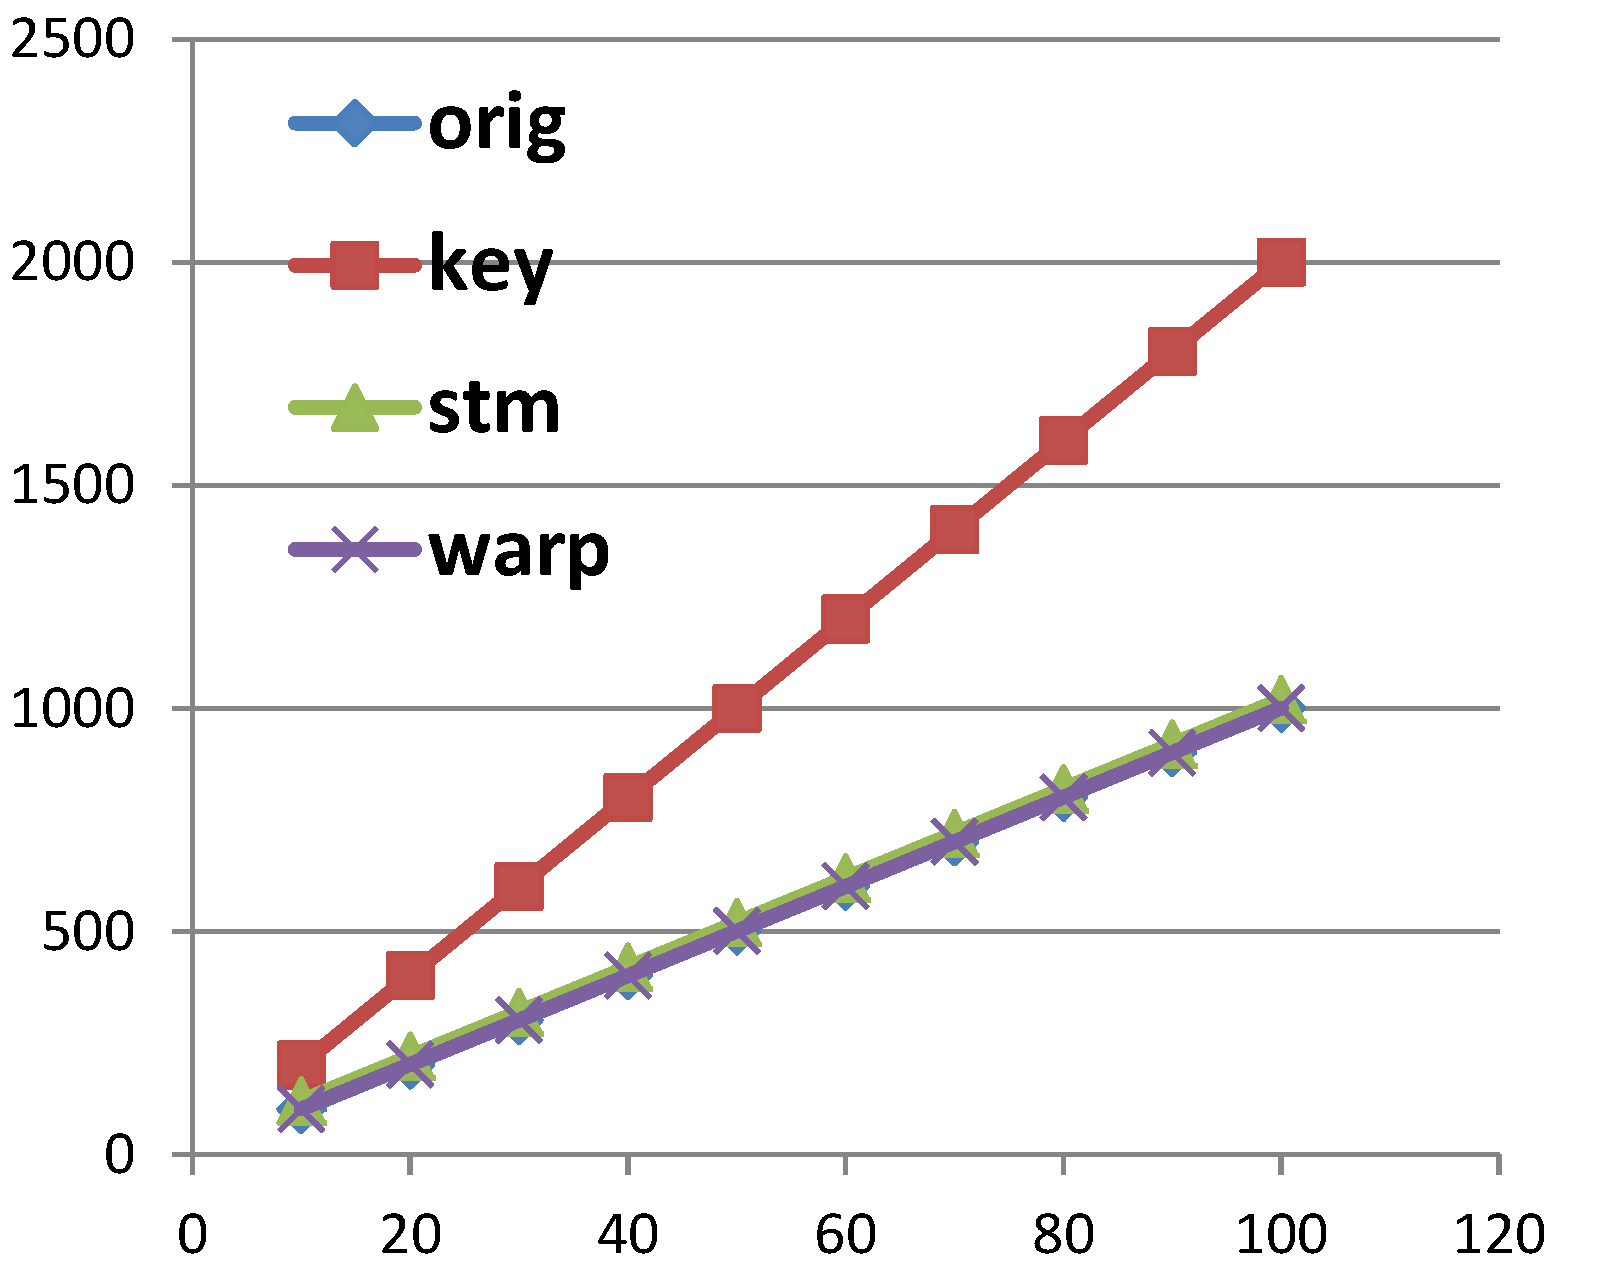
\includegraphics[width=0.33\textwidth]{../../eval/case2-iterations.png}}
\subfloat[{Case 2 with the increasing transaction duration}]{\label{fig:case2bop}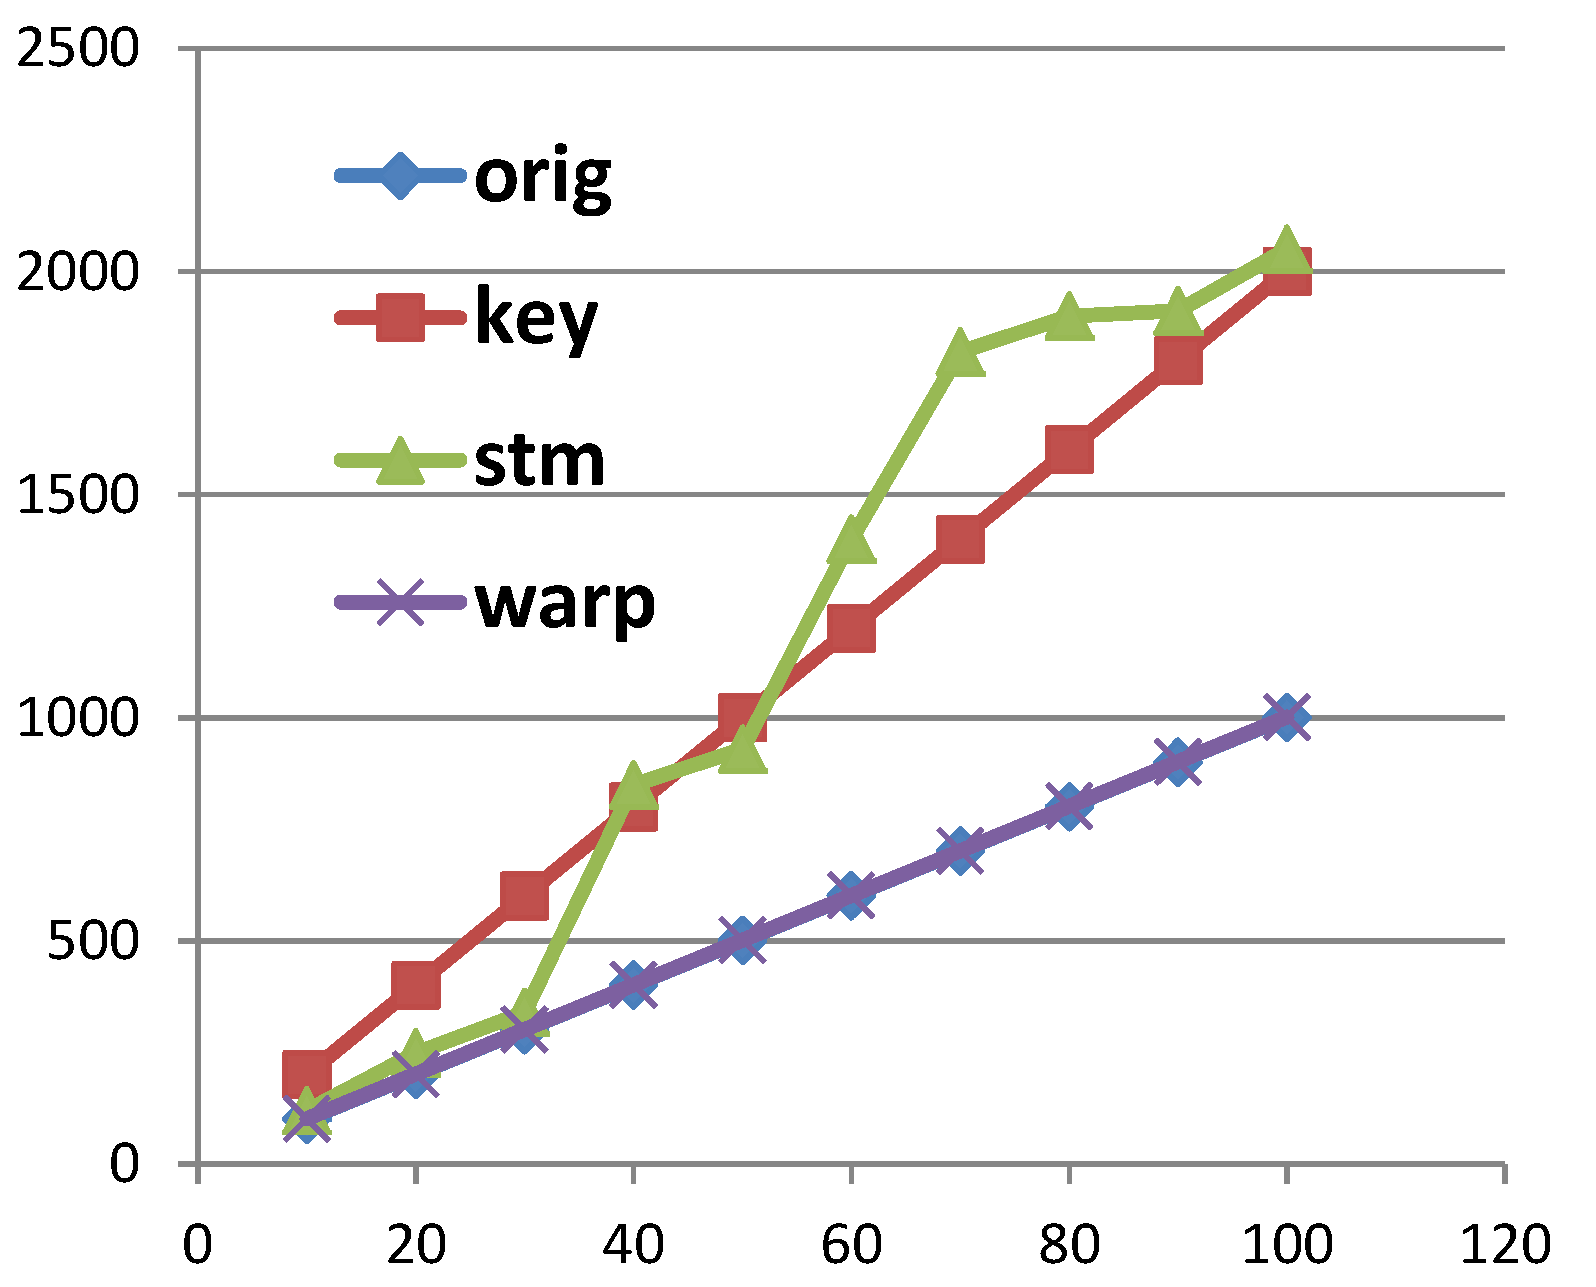
\includegraphics[width=0.33\textwidth]{../../eval/case2-bop.png}}
\\
\subfloat[{Case 3 with the increasing transaction instance number}]{\label{fig:case3iterations}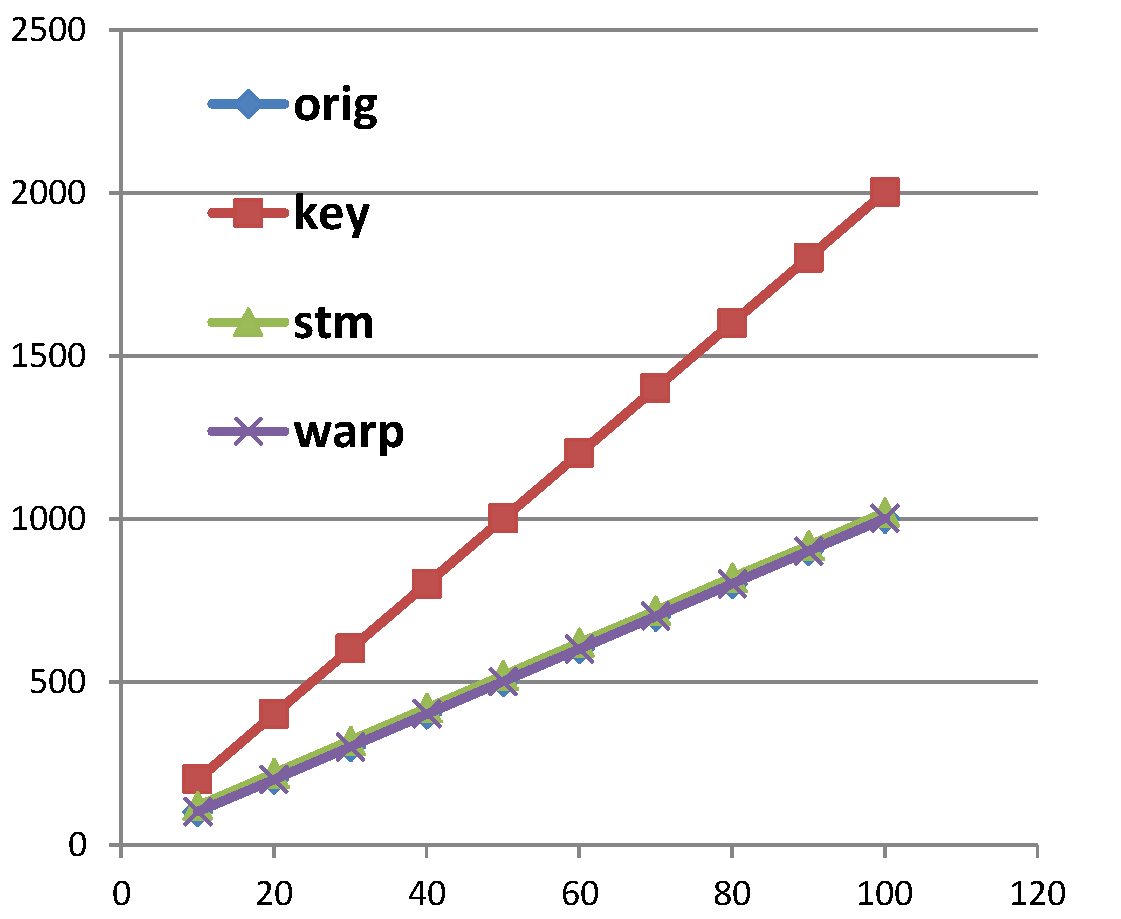
\includegraphics[width=0.33\textwidth]{../../eval/case3-iterations.png}}
\subfloat[{Case 3 with the increasing transaction duration}]{\label{fig:case3bop}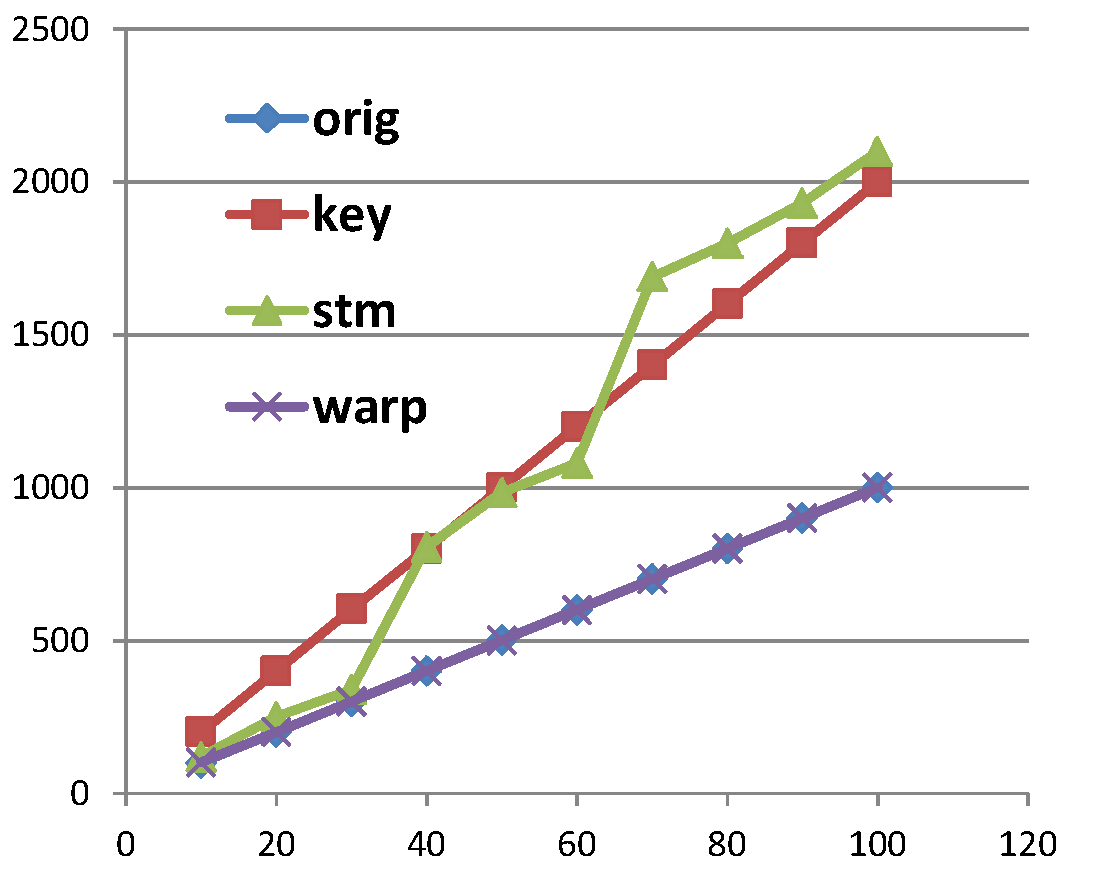
\includegraphics[width=0.33\textwidth]{../../eval/case3-bop.png}}
\\
\subfloat[{Case 4 with the increasing transaction instance number}]{\label{fig:case4iterations}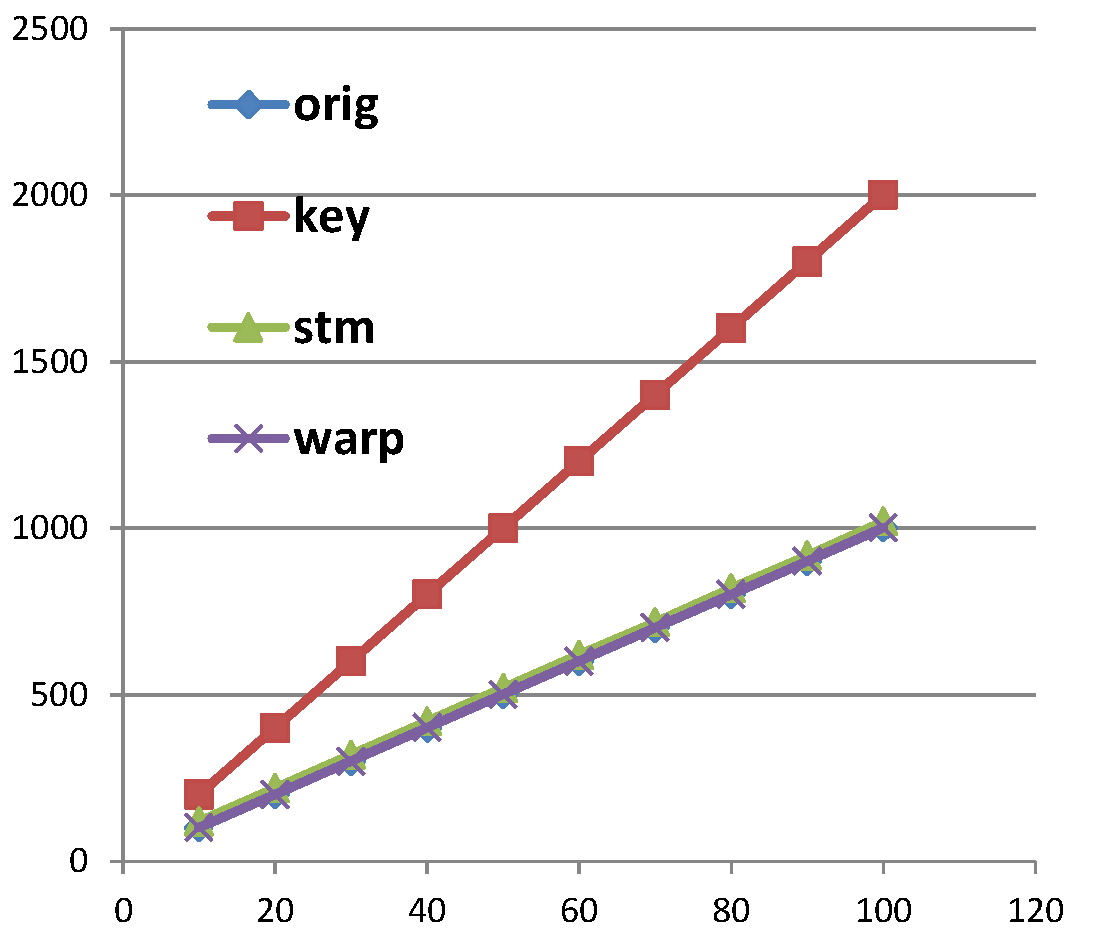
\includegraphics[width=0.33\textwidth]{../../eval/case4-iterations.png}}
\subfloat[{Case 4 with the increasing transaction duration}]{\label{fig:case4bop}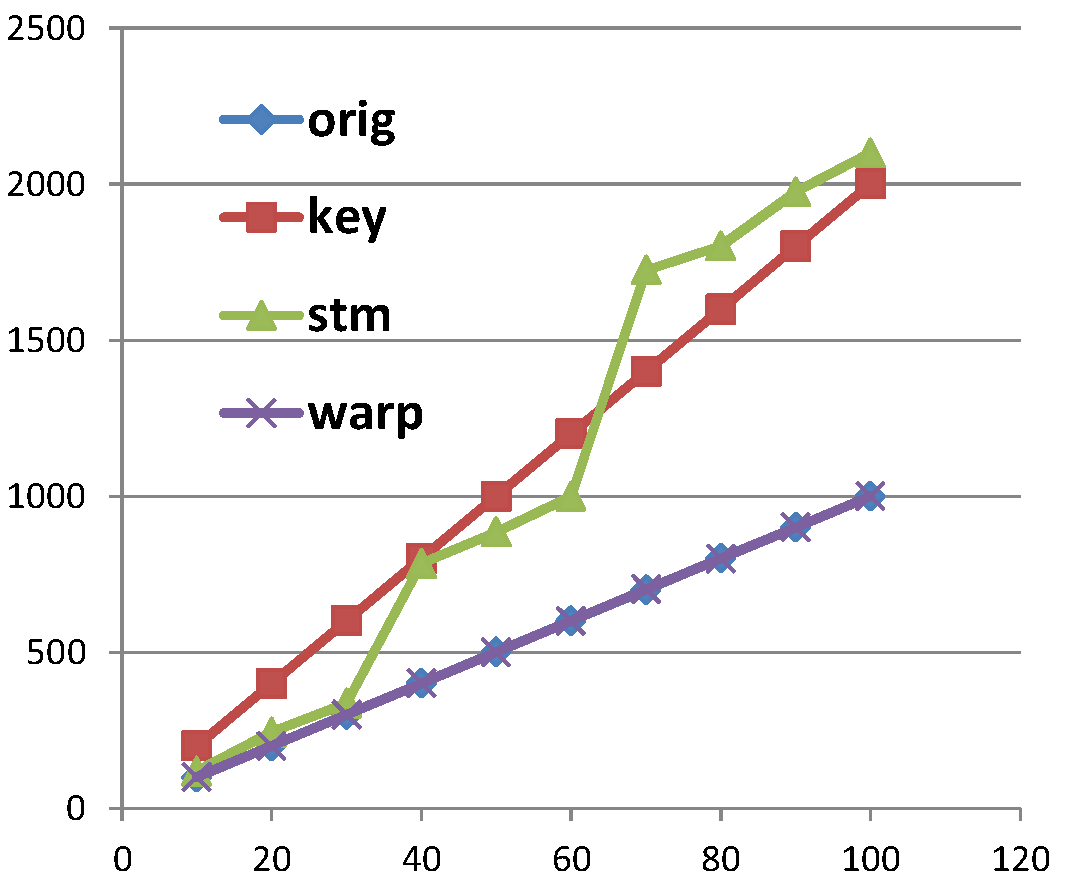
\includegraphics[width=0.33\textwidth]{../../eval/case4-bop.png}}
\\
\subfloat[{Case 5 with the increasing transaction instance number}]{\label{fig:case5iterations}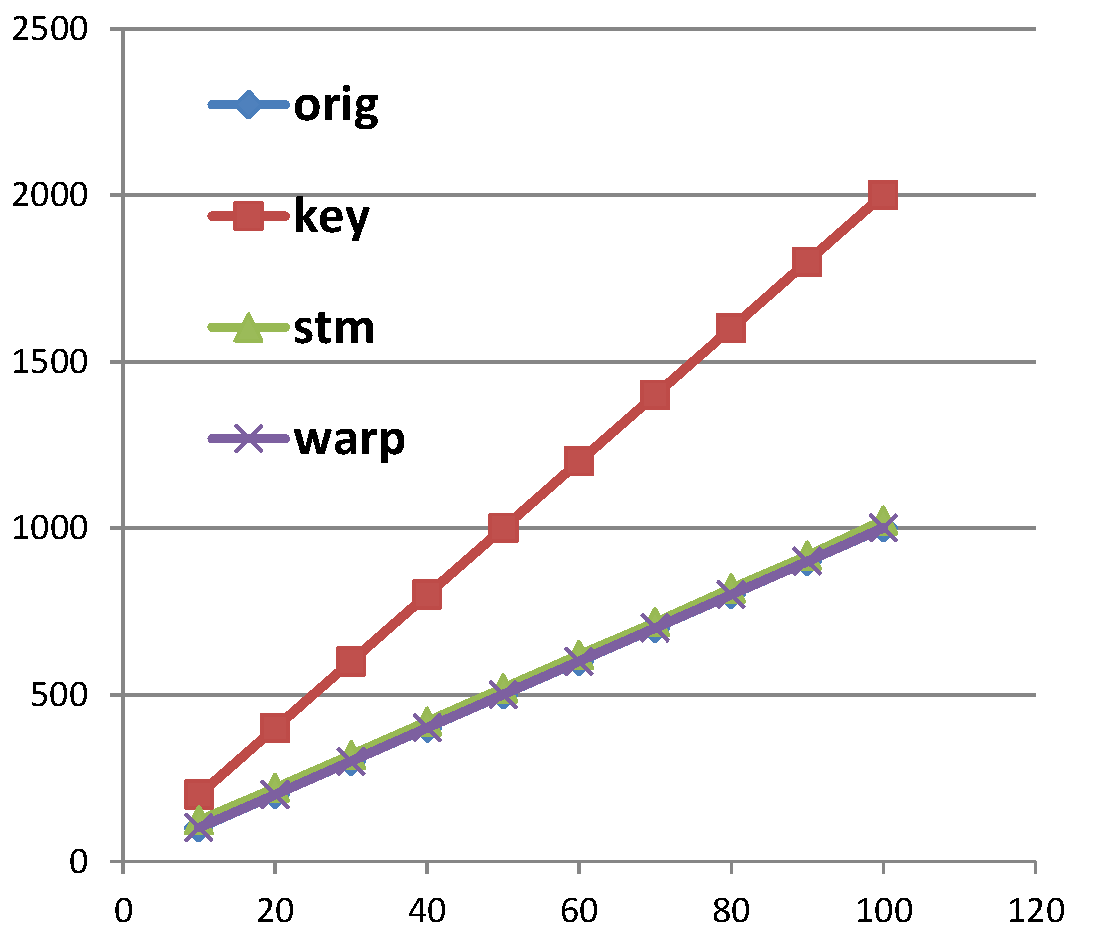
\includegraphics[width=0.33\textwidth]{../../eval/case5-iterations.png}}
\subfloat[{Case 5 with the increasing transaction duration}]{\label{fig:case5bop}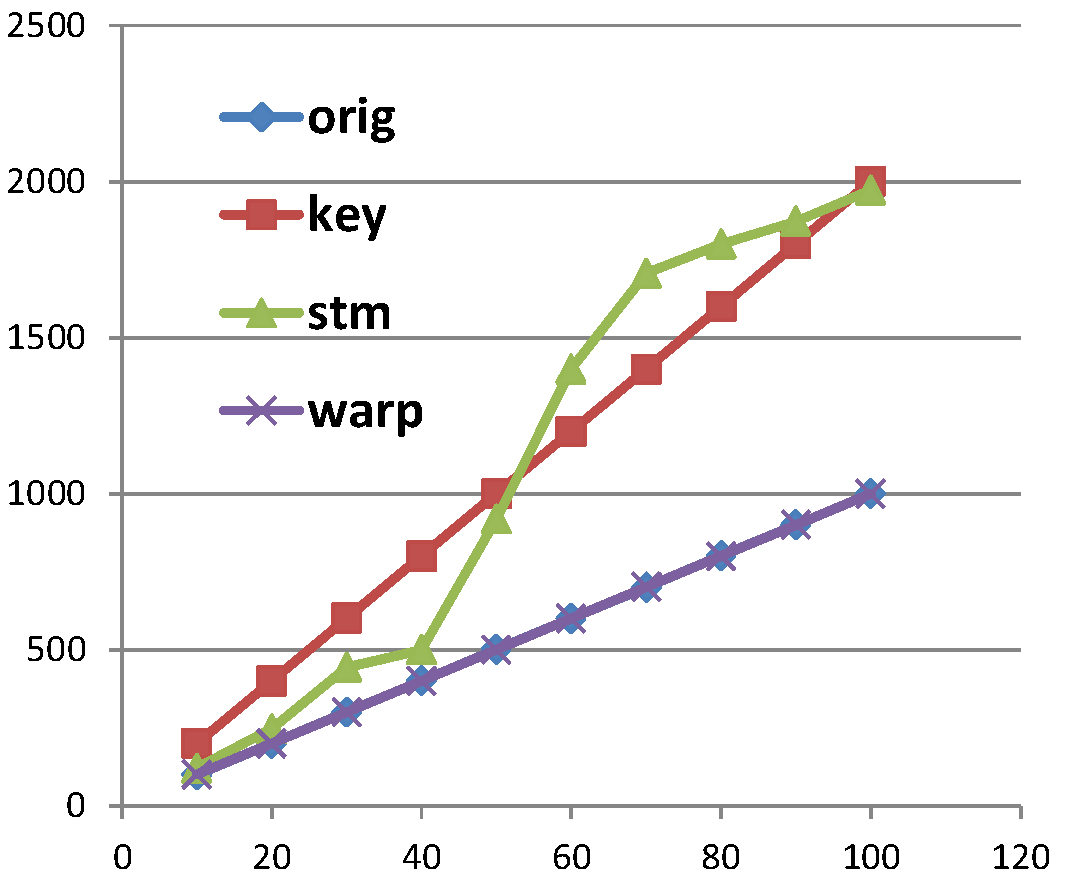
\includegraphics[width=0.33\textwidth]{../../eval/case5-bop.png}}
\caption{Performance Measurement}
\label{fig:perf}
\vspace{-1em}
\end{figure*}
